\section{Results}
\label{section:results}

In order to demonstrate the performance of our method, we conducted two sets
of tests.
In the first we simulated observables from a set of stellar parameters for a
few hundred stars using the MIST stellar evolution models and the
gyrochronology model of equation \ref{eqn:gyro}.
The ages predicted with our model were compared to the true parameters used to
generate the data.
In the second we tested our model by measuring the ages of individual stars in
the Praesepe open cluster.
% The age of Praesepe has been measured precisely because it is an ensemble of
% coeval stars with the same metallicity: a single stellar poplulation, and its
% age can be precisely established through isochrone fitting and MS turn-off.
% We adopted an age of 650 Myrs for Praesepe \citep{fossati2008}.

\subsection{Test 1: simulated stars}
For the first test we drew masses, ages, bulk metallicities, distances and
extinctions at random for 1000 stars from the following uniform distributions:
\begin{eqnarray}
& \mathrm{EEP} \sim U(198, 480) \\
% & M \sim U(0.5, 1.5)~[M_\odot] \\
& A \sim U(0.5, 14)\mathrm{~[Gyr]} \\
& F \sim U(-0.2, 0.2) \\
& D \sim U(10, 1000)~\mathrm{[pc]} \\
& A_V \sim U(0, 0.1).
\end{eqnarray}
\teff, \logg, \fhat, parallax, and apparent magnitudes $B$, $V$, $J$, $H$, $K$,
\gaia\ $G$, $G_{BP}$ and $G_{RP}$ were generated from these
stellar parameters using the MIST stellar evolution models.
We added a small amount of noise to the `observed' stellar properties in order
to reflect typical observational uncertainties.
We added Gaussian noise with a standard deviation of 25 K to \teff, 0.01 dex
to \feh\ and \logg, and 10 mmags to $B$, $V$, $J$, $H$, and $K$ magnitudes.
The noise added to Gaia $G$-band photometry ranged from
0.3 mmag for stars brighter than 13th magnitude, to 10 mmag for stars
around 20th magnitude \citep{evans2017, brown2018}.
Noise added to \gaia\ $G_{BP}$ and $G_{RP}$ bands ranged from 2 mmag for stars
brighter than 13th magnitude to 200 mmag for stars fainter than 17th.
Unphysical combinations of stellar parameters were discarded, resulting in a
final sample size of 841 simulated stars.
Figure \ref{fig:CMD_age} shows the position of these stars on an HRD
(with \logg\ on the y-axis instead of luminosity to improve the visibility of
the MS), colored by their age.
Rotation periods for FGK and early M dwarfs were generated using the
gyrochronology relation of equation \ref{eqn:gyro}.
Rotation periods for hot stars, cool stars and subgiants were generated from
Gaussian distributions (in log), with standard deviation described by the
three sigmoid functions shown in figure \ref{fig:variance}.
Based on the typical uncertainties on rotation periods in the
\citet{mcquillan2014} catalog, we added Gaussian noise with a standard
deviation of 1\% to all stellar rotation periods.
\begin{figure}
  \caption{
      The simulated star sample plotted on an HRD, colored by age
    (top panel) and rotation period (bottom panel).
    HRD positions were calculated using MIST isochrones via the {\tt
    isochrones.py} {\it Python} package and rotation periods were generated
    using equation \ref{eqn:gyro}.
    This figure was generated in a Jupyter notebook available at
    \url{https://github.com/RuthAngus/stardate/blob/master/paper/code/Simulate_data.ipynb}
}
  \centering
    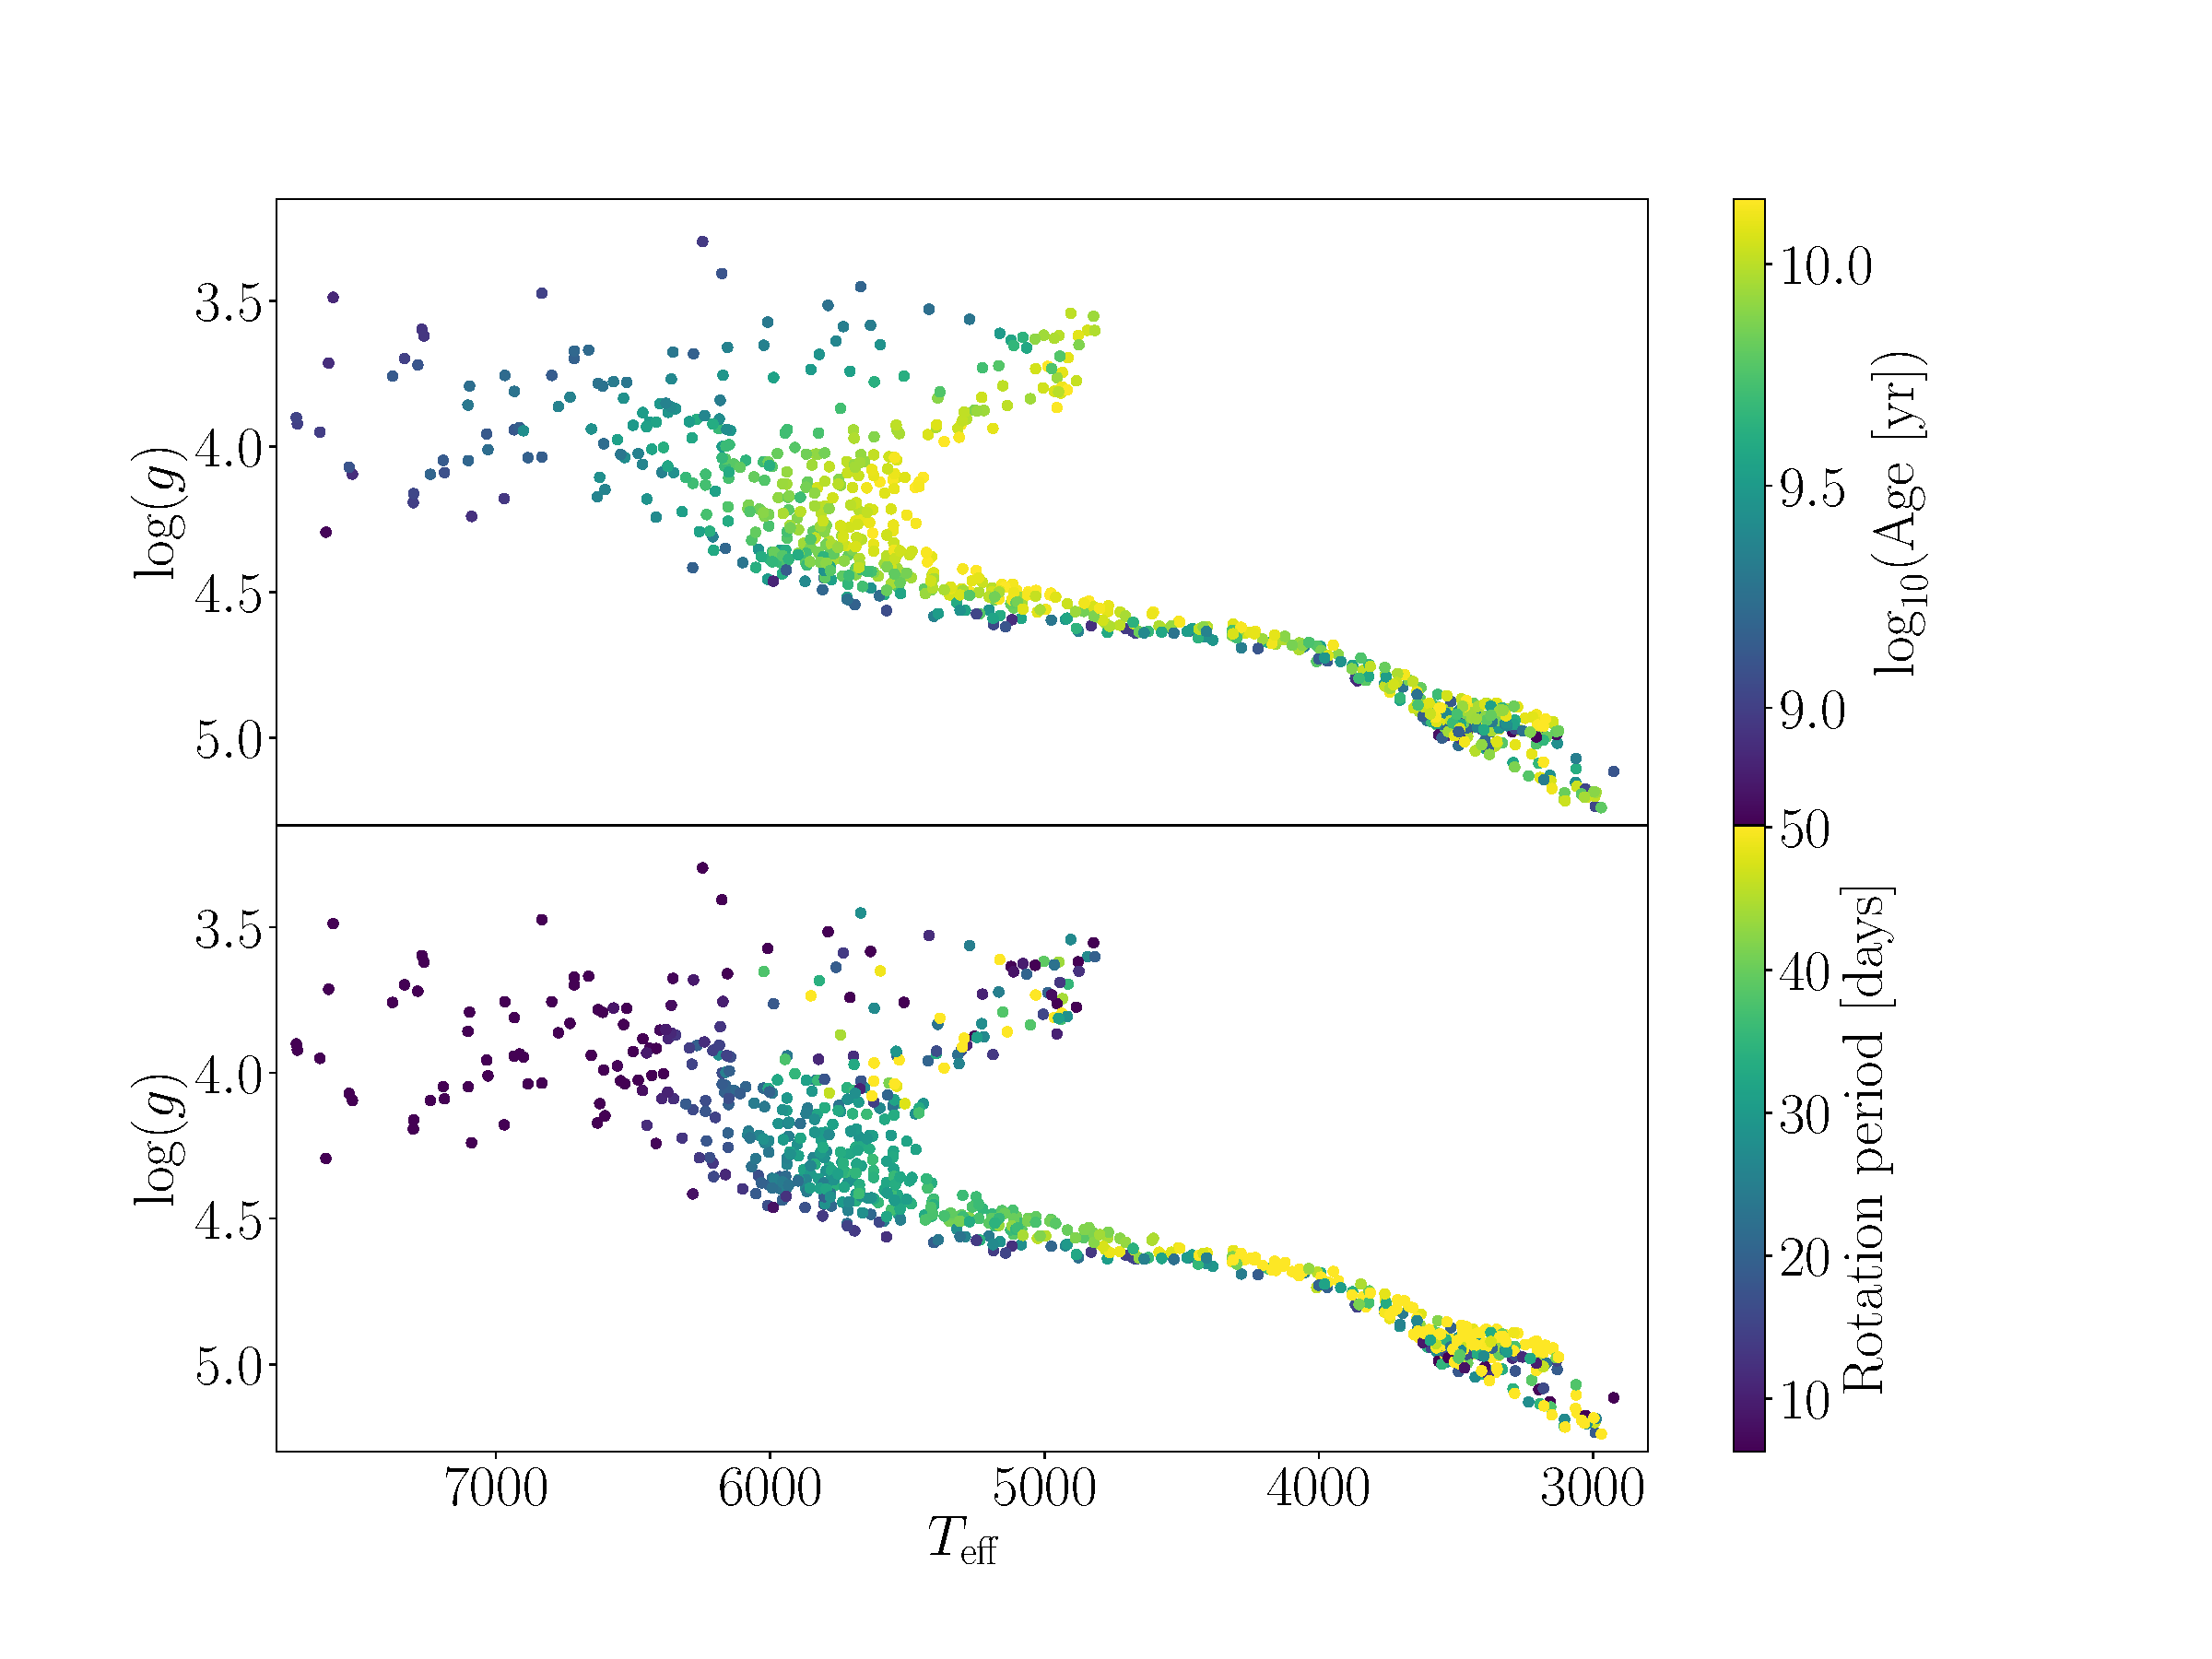
\includegraphics[width=1\textwidth]{simulated_CMD}
\label{fig:CMD_age}
\end{figure}

%   - The results
We took two approaches to inferring the ages of these simulated stars:
firstly using isochrone fitting {\it only}, and secondly using isochrone
fitting {\it combined with} a gyrochronology model (\sd).
Since the posterior PDFs of stars are often not unimodal, we found that the
choice of initial positions of the {\tt emcee} walkers influenced the final
outcome because walkers occasionally got stuck in local minima.
We found that the following set of initial parameters worked well, though not
perfectly, for FGK dwarfs but sacrificed some accuracy in subgiant ages: EEP =
330, $A = 9.56$ Gyr, $F = -0.05$, $D = 269$ pc and $A_V = 0.0$.
Figure \ref{fig:simulation_results} shows the results of combining
gyrochronology with isochrone fitting with simulated stars.
The stars' true ages are plotted against their predicted ages, with \sd\ ages
in color, and ages predicted using isochrone fitting only plotted in light
grey.
The five panels show the results for five different types of stars: late F, GK
and early M dwarfs which are still undergoing magnetic braking (Ro $<$ 2),
late F, GK and early M dwarfs that have ceased magnetic braking (Ro $>$ 2),
% hot stars ($B-V < 0.45$), cool stars ($B-V > 1.4$) and evolved stars (EEP $>$
hot stars (\gcolor\ $<$ 1.8), cool stars (\gcolor\ $>$ 2.5) and evolved stars
(EEP $>$ 454).
As expected, the low $Ro$, FGK stars show the most dramatic improvement in age
precision.
\racomment{Summary statistics rewrite in progress...}
% The median empirical age precision, the standard deviation of age posteriors
% as a percentage of age, was around 5\% for this group and the median relative
% error, defined as the absolute difference between the true and age the
% inferred age, as a percentage of the true age, was less than 2\%.
% The median error: the absolute difference between true and measured age was
% around 100 Myrs.
% In contrast, the median empirical precision of ages measured using only
% isochrone fitting was 50\% and the median error was 1.3 Gyr in absolute units,
% or 30\%.
% Ages measured for FGK stars by combining gyrochronology and isochrone fitting
% with \sd\ were 10 times more precise than ages measured with isochrone
% fitting.
% Even though the group of old FGK stars with large Rossby numbers have stopped
% magnetic braking, their rotation periods are still age-informative and
% relatively precise ages were measured for these stars with \sd.
% The median age precision for this group was 10\% with \sd\ and 22\% with
% isochrone fitting.
% The median age error was 500 Myr/5\% with \sd\ and 1.3 Gyr/16\% with isochrone
% fitting.
% Ages measured with \sd\ were around twice more precise than ages measured with
% isochrone fitting only, so although these stars have stopped spinning down,
% their rotation periods are still age-informative when paired with stellar
% evolution models.
% There is a tendency for the ages of these stars to be slightly underestimated
% however.
% % The median accuracy of hot star ages stayed roughly constant with \sd,
% % relative to isochrone fitting only (from a median error of 510 Myr to 560 Myr)
% % because of issues with sampling the posterior PDFs.
% % Adding gyrochronology to the age model creates a more multimodal posterior PDF
% % which makes sampling more difficult, leading to some highly inaccurate age
% % measurements at very high and very low ages.
% There was only a very slight improvement the precision of cool star, hot star
% and subgiant ages measured with \sd\ vs. isochrone
% fitting only.
% % This is expected because the rotation periods of these stars do not contain
% % information about stellar ages.
% For the whole sample, an overall median age precision of 10\% was provided by
% \sd\ (down from 28\% for isochrone fitting only), a median absolute error of
% 500 Myrs (down from 1.3 Gyrs), and a relative error of 7\% (down from 23 \%).
% % On average, the ages of {\it all} FGKM dwarfs and subgiants were 3$\times$
% % more precise when their rotation periods were used to infer their ages.
\begin{figure}
  \caption{
The true vs. predicted ages of simulated stars.
    Ages calculated by combining gyrochronology
    and isochrone fitting with \sd are shown in color and ages calculated with
    isochrone fitting only are shown in gray.
The five panels show the results for five different groups of stars: low $Ro$
late F, GK and early M dwarfs, high $Ro$ late F, GK and early M dwarfs, early
    % F stars (B-V $<$ 0.45), late M dwarfs (B-V $>$ 1.4) and subgiants
    F stars (\gcolor\ $<$ 0.56), late M dwarfs (\gcolor\ $>$ 2) and subgiants
    (EEP $>$ 454).
Gyrochronology is highly effective for low $Ro$ late F, GK and early M dwarfs
and somewhat effective for high $Ro$ late F, GK and early M dwarfs.
Ages for other groups were improved slightly but not substantially.
% Outliers are caused by multimodal posterior PDFs and imperfect MCMC sampling.
}
  \centering
    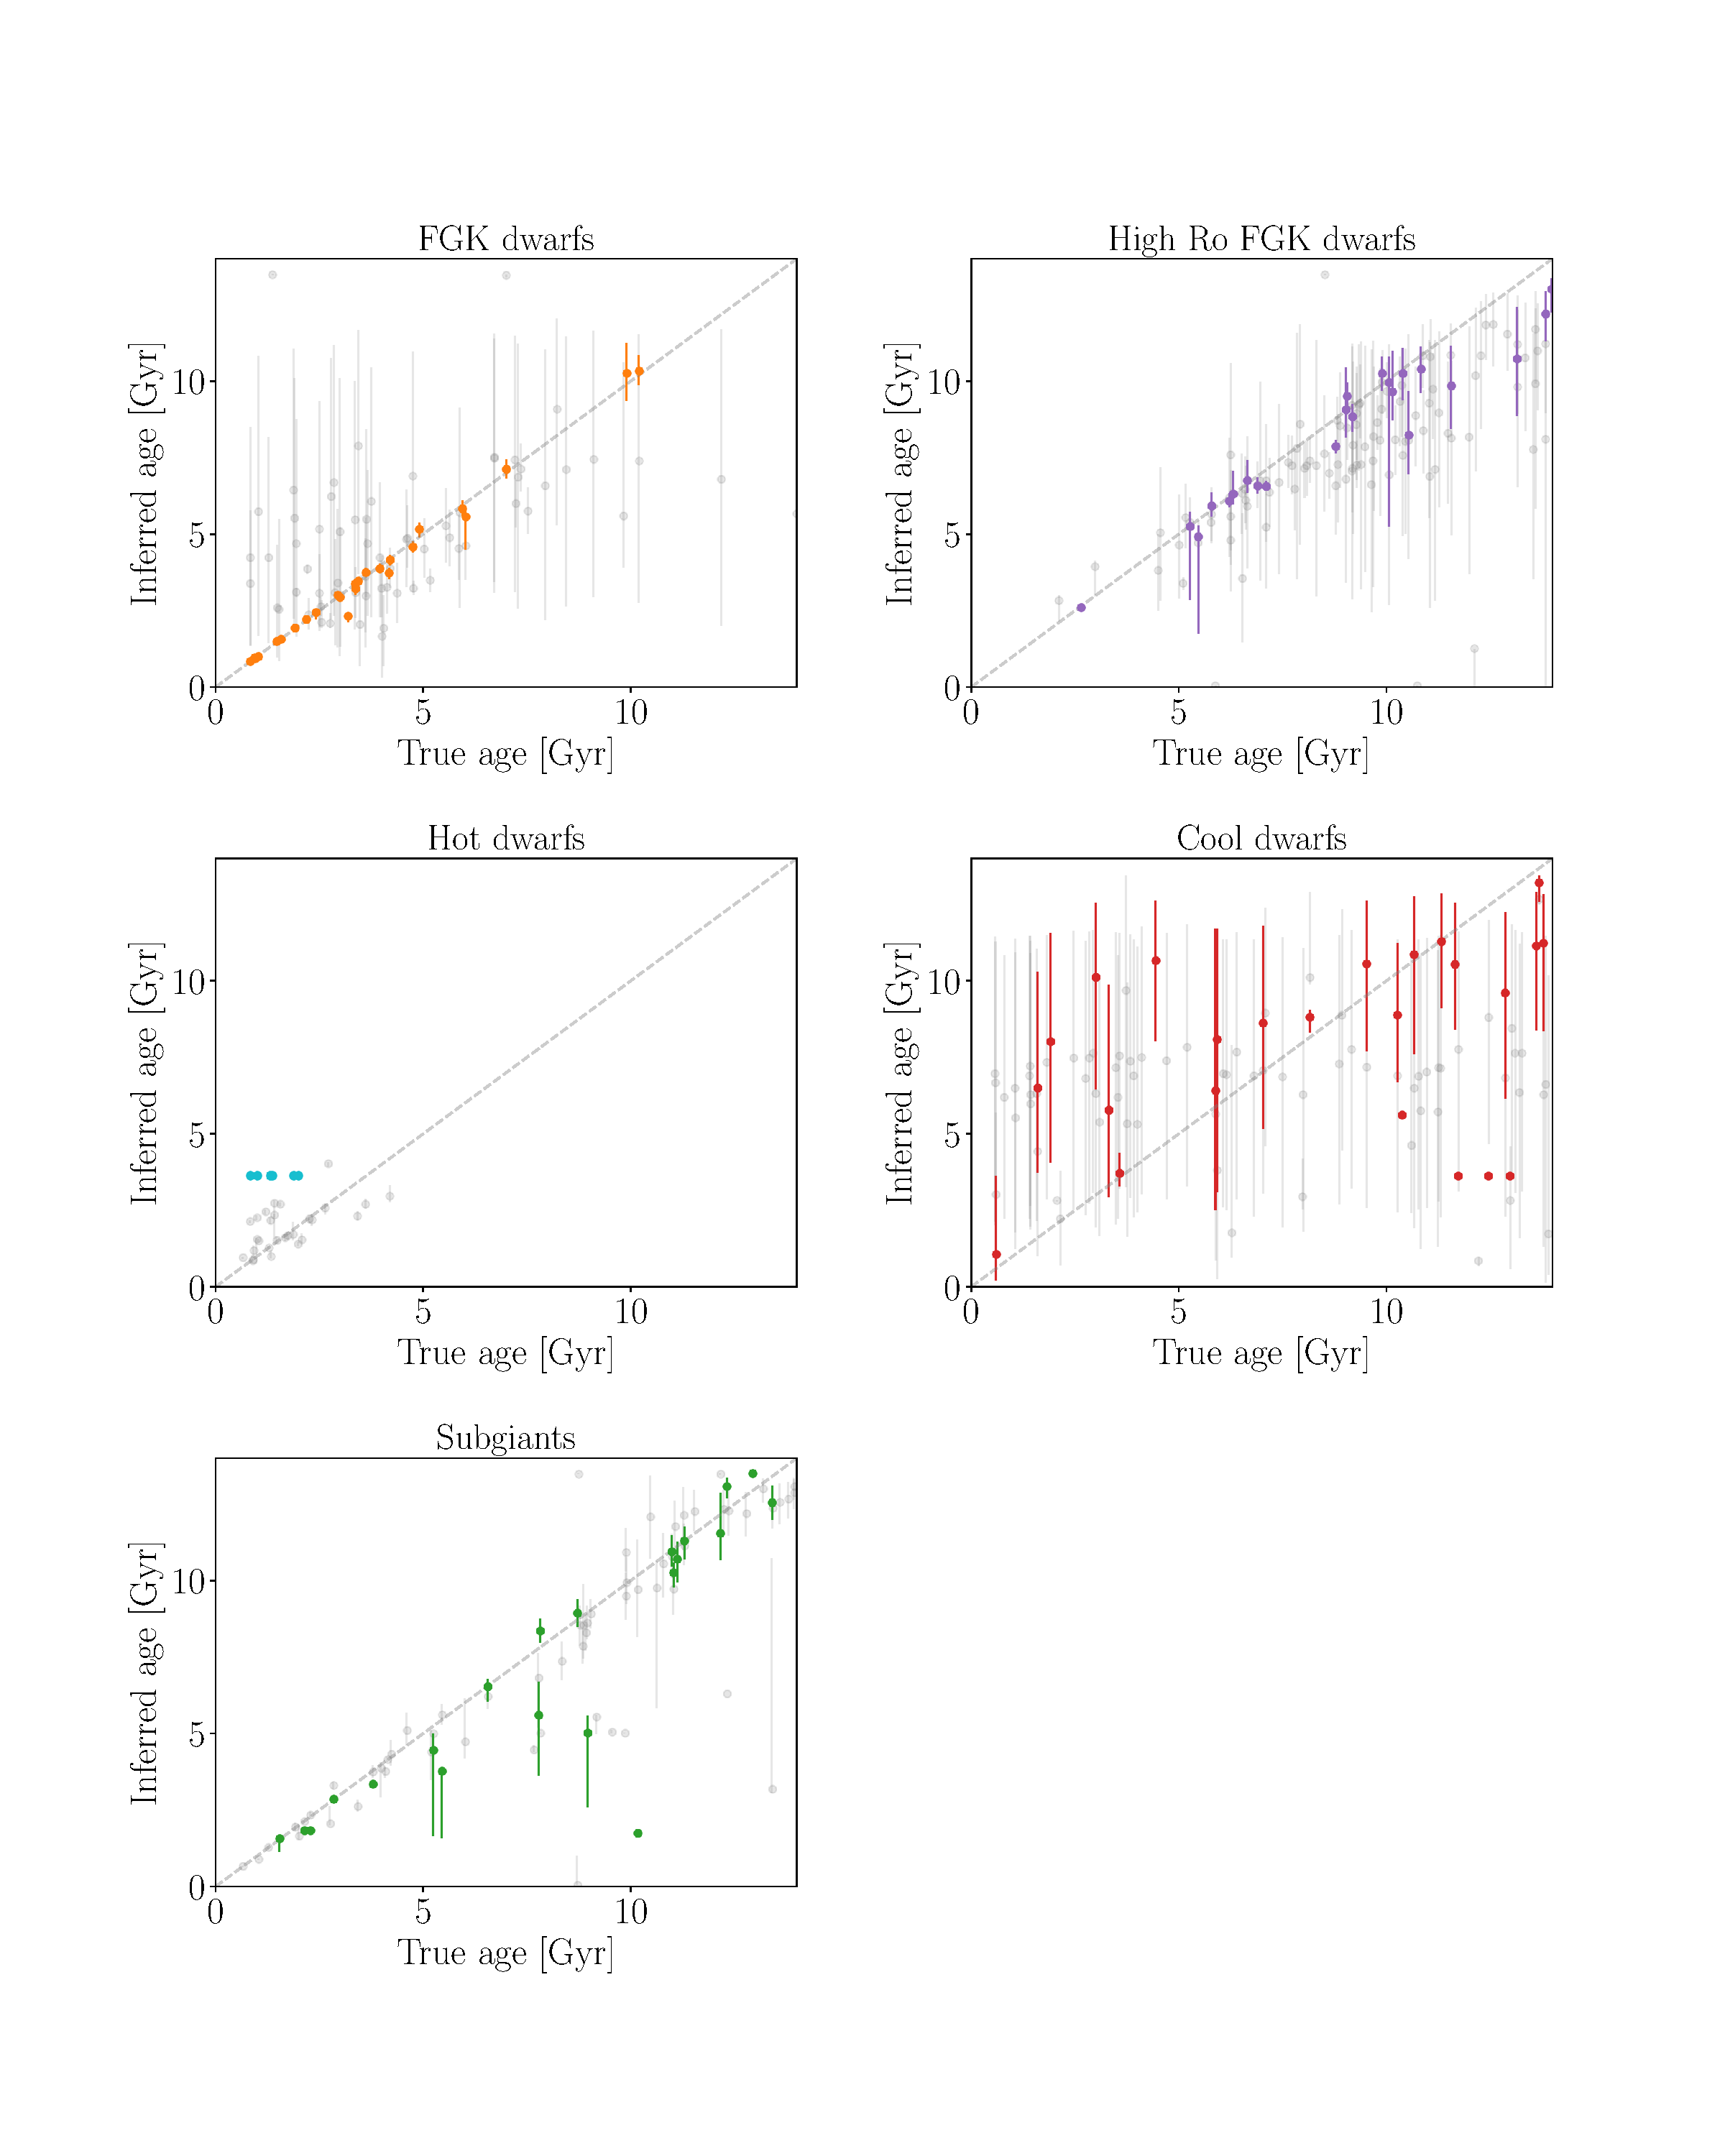
\includegraphics[width=1\textwidth]{simulation_results}
\label{fig:simulation_results}
\end{figure}

Figure \ref{fig:precision} shows the simulated stars on an HRD, with
points colored by the relative precision of their predicted ages.
% \logg\ is plotted the y-axis instead of luminosity because the MS spreads out
% more in \teff-\logg\ space and it is easier to differentiate young and old
% stars.
The top panel shows the precision of ages calculated using both gyrochronology
and isochrone fitting with \sd\ and the bottom panel shows the precision of
ages calculated with isochrone fitting only.
Although these uncertainties are noisy (they are computed from the standard
deviation of the age posteriors) they show that combining gyrochronology and
isochrone fitting significantly improves age precision on the MS
\begin{figure}
  \caption{
Simulated stars on an HRD, colored by their relative age precision
    using gyrochronology and isochrone fitting via \sd\ (top panel) and
    isochrone fitting only (bottom panel).
Combining gyrochronology with isochrone fitting significantly improves stellar
    age precision on the MS.
% Gyrochronology is responsible for the high precision of ages measured for
%     young FGK stars (stars in the upper left panel of figure
%     \ref{fig:simulation_results}.
% The ages of old FGK stars with $Ro > $2 are slightly less precise as these
%     stars have stopped spinning down and their rotation periods are not
%     information-rich.
Isochrone fitting provides precise ages for hot stars and subgiants and the
    rotation periods of these stars are relatively uninformative, so
    gyrochronology does not significantly improve their age precision.
The ages of late M dwarfs are highly imprecise because their ages are not well
    determined by either their rotation periods or their position on the HRD
    or CMD.
}
  \centering
    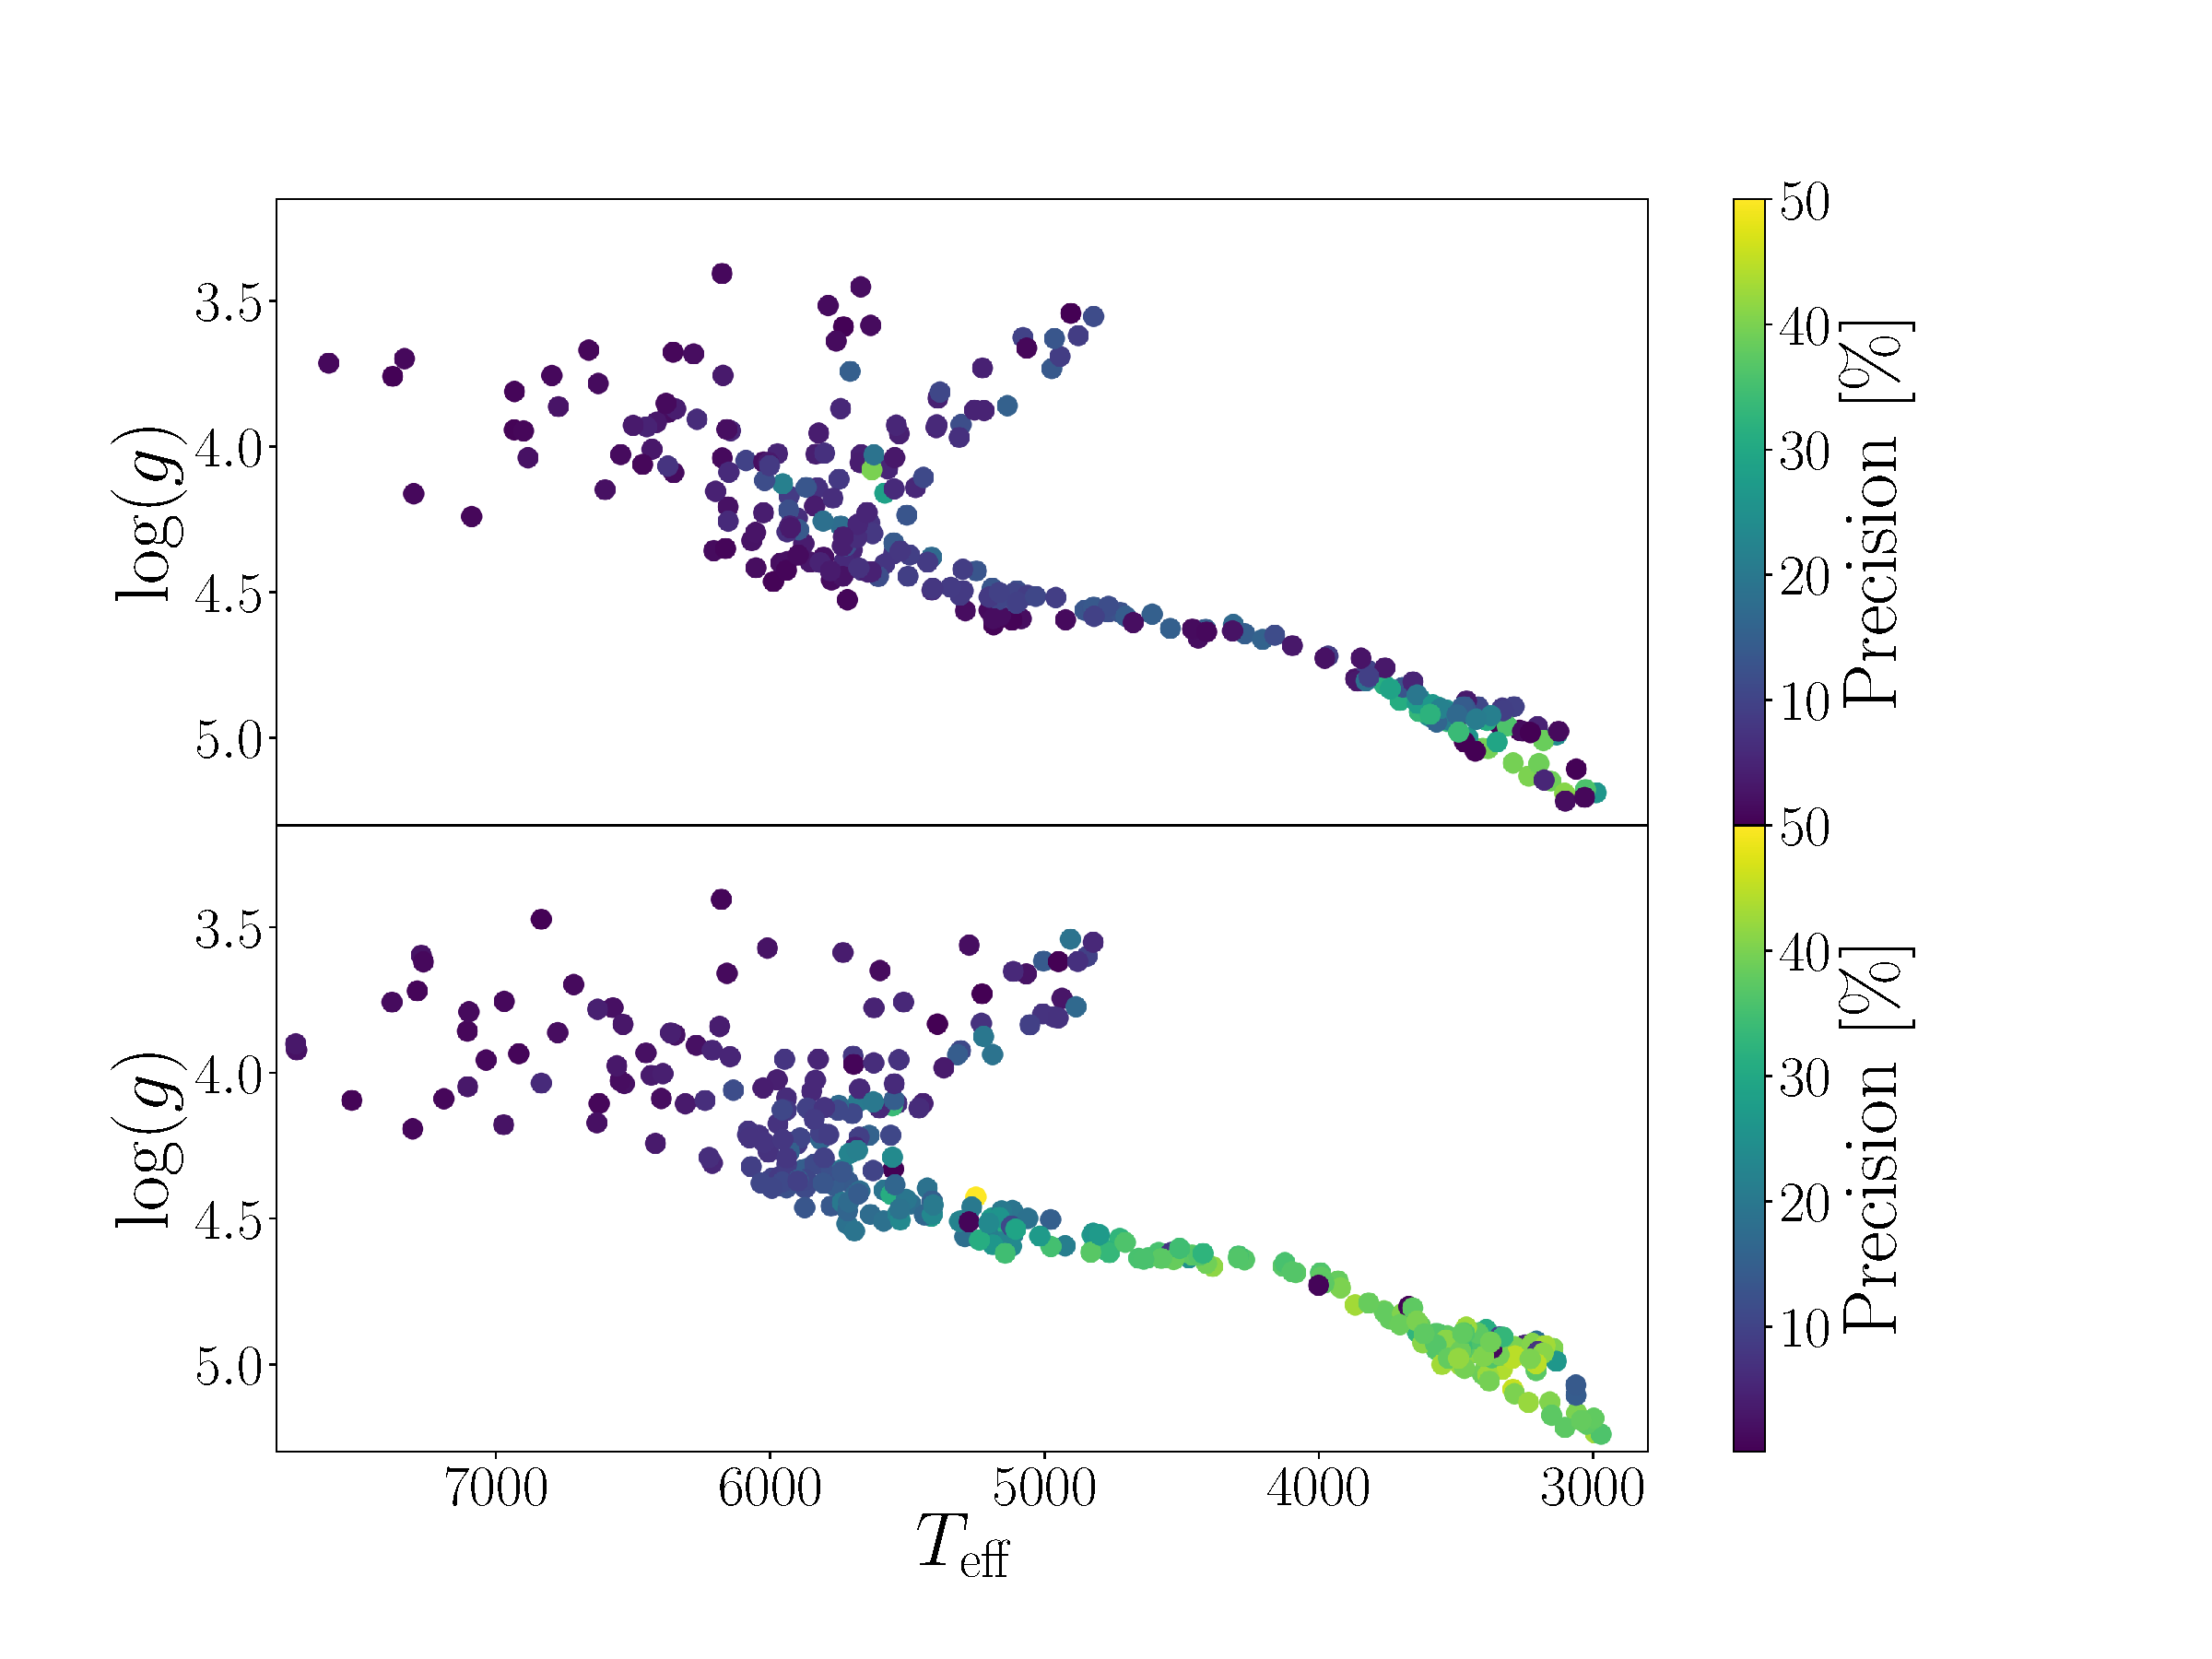
\includegraphics[width=1\textwidth]{precision_plot}
\label{fig:precision}
\end{figure}

% \begin{figure}
%   \caption{
% The sample of simulated stars on an HRD, colored by the difference
%     between their true age and their measured age (the age error).
% }
%   \centering
%     \includegraphics[width=1\textwidth]{error_plot}
% \label{fig:accuracy}
% \end{figure}


% We're cheating here.
% Figure \ref{gyro_only} demonstrates the results of inferring ages using
% rotation periods only, and this illustrates why the combination of isochronal
% and gyrochronal ages is so precise: almost all this precision comes from
% rotation periods.
This simulation experiment is optimistic because data were simulated from the
same gyrochronology model used to infer ages, so the results for FGK dwarfs
are extremely accurate by design.
% Secondly, we simulated data without any noise or any additional instrinsic
% scatter for FGK dwarfs, resulting in ages with better precision than can be
% expected for real stars.
% Inaccuracies would arise if the gyrochronology model was incorrect or poorly
% calibrated in some areas of parameter space and additional imprecision would
% arise if excess intrinsic scatter were built into the gyrochronology model
% and/or the observations.
\sd\ can provide precise ages with the caveat that the currently implemented
gyrochronology model is not perfectly calibrated and ages will only be as
accurate as the model.
We leave further recalibration of gyrochronology models for a future exercise
since, in this work, we were mostly interested in testing the results of
combining existing gyrochronology relations with isochrone fitting.
% The above experiment demonstrates that building gyrochronology into stellar
% evolution models results in much more precise age predictions, as predicted by
% information theory.

% TEST 2: Clusters
%-----------------------------------------------------------------------------
%   - The cluster data
\subsection{Test 2: the Praesepe Cluster}
In order to test our model on real stars with known ages, we selected a sample
of stars in the Praesepe open cluster.
The ages of open clusters can be measured much more precisely than field stars
because they formed from the same molecular cloud at the same time and
therefore have the same metallicity and age (to within a few million years).
Stars with the same metallicity and age fall on the same isochrone, and
provide a $N^{-1/2}$ decrease in age uncertainty where N is the number of
cluster stars.
Single stellar populations also allow main sequence turn off to be identified
which provides a large amount of age information.
We compiled rotation periods, \Gaia\ photometry and \gaia\ parallaxes for
members of Praesepe, a 650 Myr cluster \citep{fossati2008}.
We chose Praesepe because it is relatively tightly clustered on the sky and
many of its members were targeted in a single \ktwo\ campaign, from which
rotation periods were measured via light curve frequency analysis
\citep{douglas2017, rebull2017}.
We identified Praesepe members with measured rotation periods from the
\citet{douglas2017} catalog in the \ktwo-\gaia\ crossmatch catalog provided at
\url{https://gaia-kepler.fun/}.
This catalog cross-matched the EPIC catalog \citep{huber2016} with with the
Gaia DR2 catalog \citep{brown2018}, using a 1'' search radius.
The result was a sample of 757 stars with rotation periods, parallaxes and
\gaia\ $G$, $G_{BP}$ and $G_{RP}$-band photometry\footnote{This analysis was
performed in a Jupyter notebook available here:
\url{
https://github.com/RuthAngus/stardate/blob/master/paper/code/Praesepe.ipynb}}.
% Equal-mass binaries were identified based on their CMD position and excluded
% because these stars usually do not follow a simple gyrochronology relation.
% We also excluded late M dwarfs because their rotation periods do not provide a
% strong prediction of their age.
Figure \ref{fig:praesepe} shows the rotation periods of Praesepe members as a
function of their \gaia\ \gcolor\ colors with the new gyrochronology model fit
to it (black dashed lines) and an older gyrochronology relation
\citep{angus2015}.
% This relation clearly does not provide a good fit to the Praesepe cluster.
% This is because the relation was calibrated using a number of clusters, and
% the model represents a combination of the different clusters' period-color
% relations.
% In addition, the model does not described the M dwarfs well because these
% Praesepe rotation periods were measured from \ktwo\ light curves
% \citep{douglas2017}, published after this gyrochronology relation was
% calibrated \citet{angus2015}.
% The rotational behaviour of M dwarfs observed in this cluster has not yet been
% incorporated into gyrochronology models.
Praesepe has several rotational outliers: stars with rotation periods much
higher or lower than the majority of data points.
Some of these outliers have excess luminosity which is suggestive of binarity
and others are likely to be lower mass-ratio binaries (Douglas \etal, in prep).
% FGK and early M stars, that lie tightly on the Praesepe isochrone and do not
% show excess luminosity suggestive of being a binary are shown as solid blue
% points.
% We only applied \sd\ to these stars because the purpose of this test was to
% demonstrate that it can predict accurate ages for stars that fall on the
% gyrochronology relation.
Because the gyrochronology model does not capture the rotational behavior of
these outliers, \sd\ is not designed to predict precise ages for binary stars
or other outliers.
% The late F, GK and early M dwarfs (\gcolor\ $<$ 2.4) which fall on a `rotational main
% sequence' are shown as blue points and the late M dwarfs (\gcolor\ $>$ 2.4)
% whose rotation periods are not well determined by their age and color are
% shown as orange open circles.
% We excluded the late M dwarfs (orange circles with \gcolor\ $>$ 2.4) from this
% analysis since they do not follow a simple gyrochronology relation however, we
% included more massive outliers (orange circles with \gcolor\ $<$ 2.4) in order
% to provide a complete picture of the precision and accuracy of gyrochronology
% applied to Praesepe.
% \begin{figure}
%   \caption{
%     The rotation periods of Praesepe members \citep{douglas2016},
%     vs. their \Gaia\ colors (\gcolor) with a broken power law model fit to
%     Praesepe.
%     Shaded regions show the 1$\sigma$ range of the stochastic rotation period
%     model for M dwarfs and hot stars.
%     The rotation periods of these stars are modelled as a broad Gaussian.
%     This model does not perfectly represent Praesepe because it does not
%     account for outliers.
%     This figure was generated in a Jupyter notebook available at this
%     url:\url{https://github.com/RuthAngus/stardate/blob/master/paper/code/Fitting_Praesepe.ipynb}
% }
%   \centering
%     \includegraphics[width=1\textwidth]{Praesepe.pdf}
% \label{fig:praesepe}
% \end{figure}

Figure \ref{fig:praesepe_results} shows the posterior PDFs over age for the
FGK and early M dwarf members of the praesepe cluster where each star was
treated as a field star.
Age posteriors calculated with \sd\ are shown in blue and, for comparison, age
posteriors calculated using isochrone fitting only are shown in orange.
\gaia\ colors (\gcolor), \gaia\ apparent magnitude ($G$), \gaia\ parallaxes
and rotation periods were used the observable properties.
The blue PDFs are more tightly clustered around the established age of
Praesepe ($\sim650$Myrs, shown as a dashed vertical line) than the orange PDFs
because rotation periods are extremely age-informative for these stars.
However, the accuracy of these ages is limited because of the limited accuracy
of the gyrochronology model.
Until the gyrochronology model is improved to incorporate rotational outliers
and binaries, ages calculated with \sd\ should be interpreted with caution.
% Figure \ref{fig:praesepe} shows two sets of gyrochronology models: one
% calibrated using several open clusters, asteroseismic stars and the Sun
% \citep{angus2015}, which was used to infer the ages of Praesepe but clearly
% does not provide a perfect fit to this cluster (solid gray line), and one fit
% to Praesepe and the Sun only, as described in section
% \ref{section:motivation}, that was used to calculate the Fisher information
% (dashed black line).
% We did not account for extinction in our analysis since Praesepe is relatively
% nearby (around 180 parsecs) so reddening from dust is minimal.
% The age of each Praesepe member was inferred using both of these
% gyrochronology models: the legacy model of equation \ref{eq:gyro} and the
% Praesepe model of equation \ref{eq:new_gyro}.
% This exercise is not designed to test one gyrochronology model against
% another: the model fit to the Praesepe data will provide a better age
% prediction by design, as the legacy model was fit to number of clusters at
% once.
% The point of this exercise is to show how precise gyrochronology could be if
% a {\it perfect} model was used.
% The age of each Praesepe member was inferred using our combined stellar
% evolution and gyrochronology model.
% We did not force the cluster members to have the same age since the aim of
% this experiment was to reveal the precision and accuracy of our method by
% quantifying the level of scatter in our predicted ages and identifying regions
% of parameter space where the ages deviate from the established age for
% Praesepe.
\begin{figure}
  \caption{
Posterior PDFs over the ages of members of the 650 Myr Praesepe cluster.
The blue posteriors were recovered with \sd, by combining \gaia\ apparent
    magnitudes ($G$, $G_BP$ and $G_RP$) and parallaxes with their photometric,
    \ktwo\ rotation periods.
The orange posteriors were obtained for the same stars using isochrone fitting
    with \gaia magnitudes and parallaxes.
Each star was treated as a single field star.
The blue posteriors are more tightly peaked and clustered around the true age
of the cluster because rotation periods add age information.
These blue posteriors are not always accurate because they reflect the scatter
within rotation periods in the Praesepe cluster.
}
  \centering
    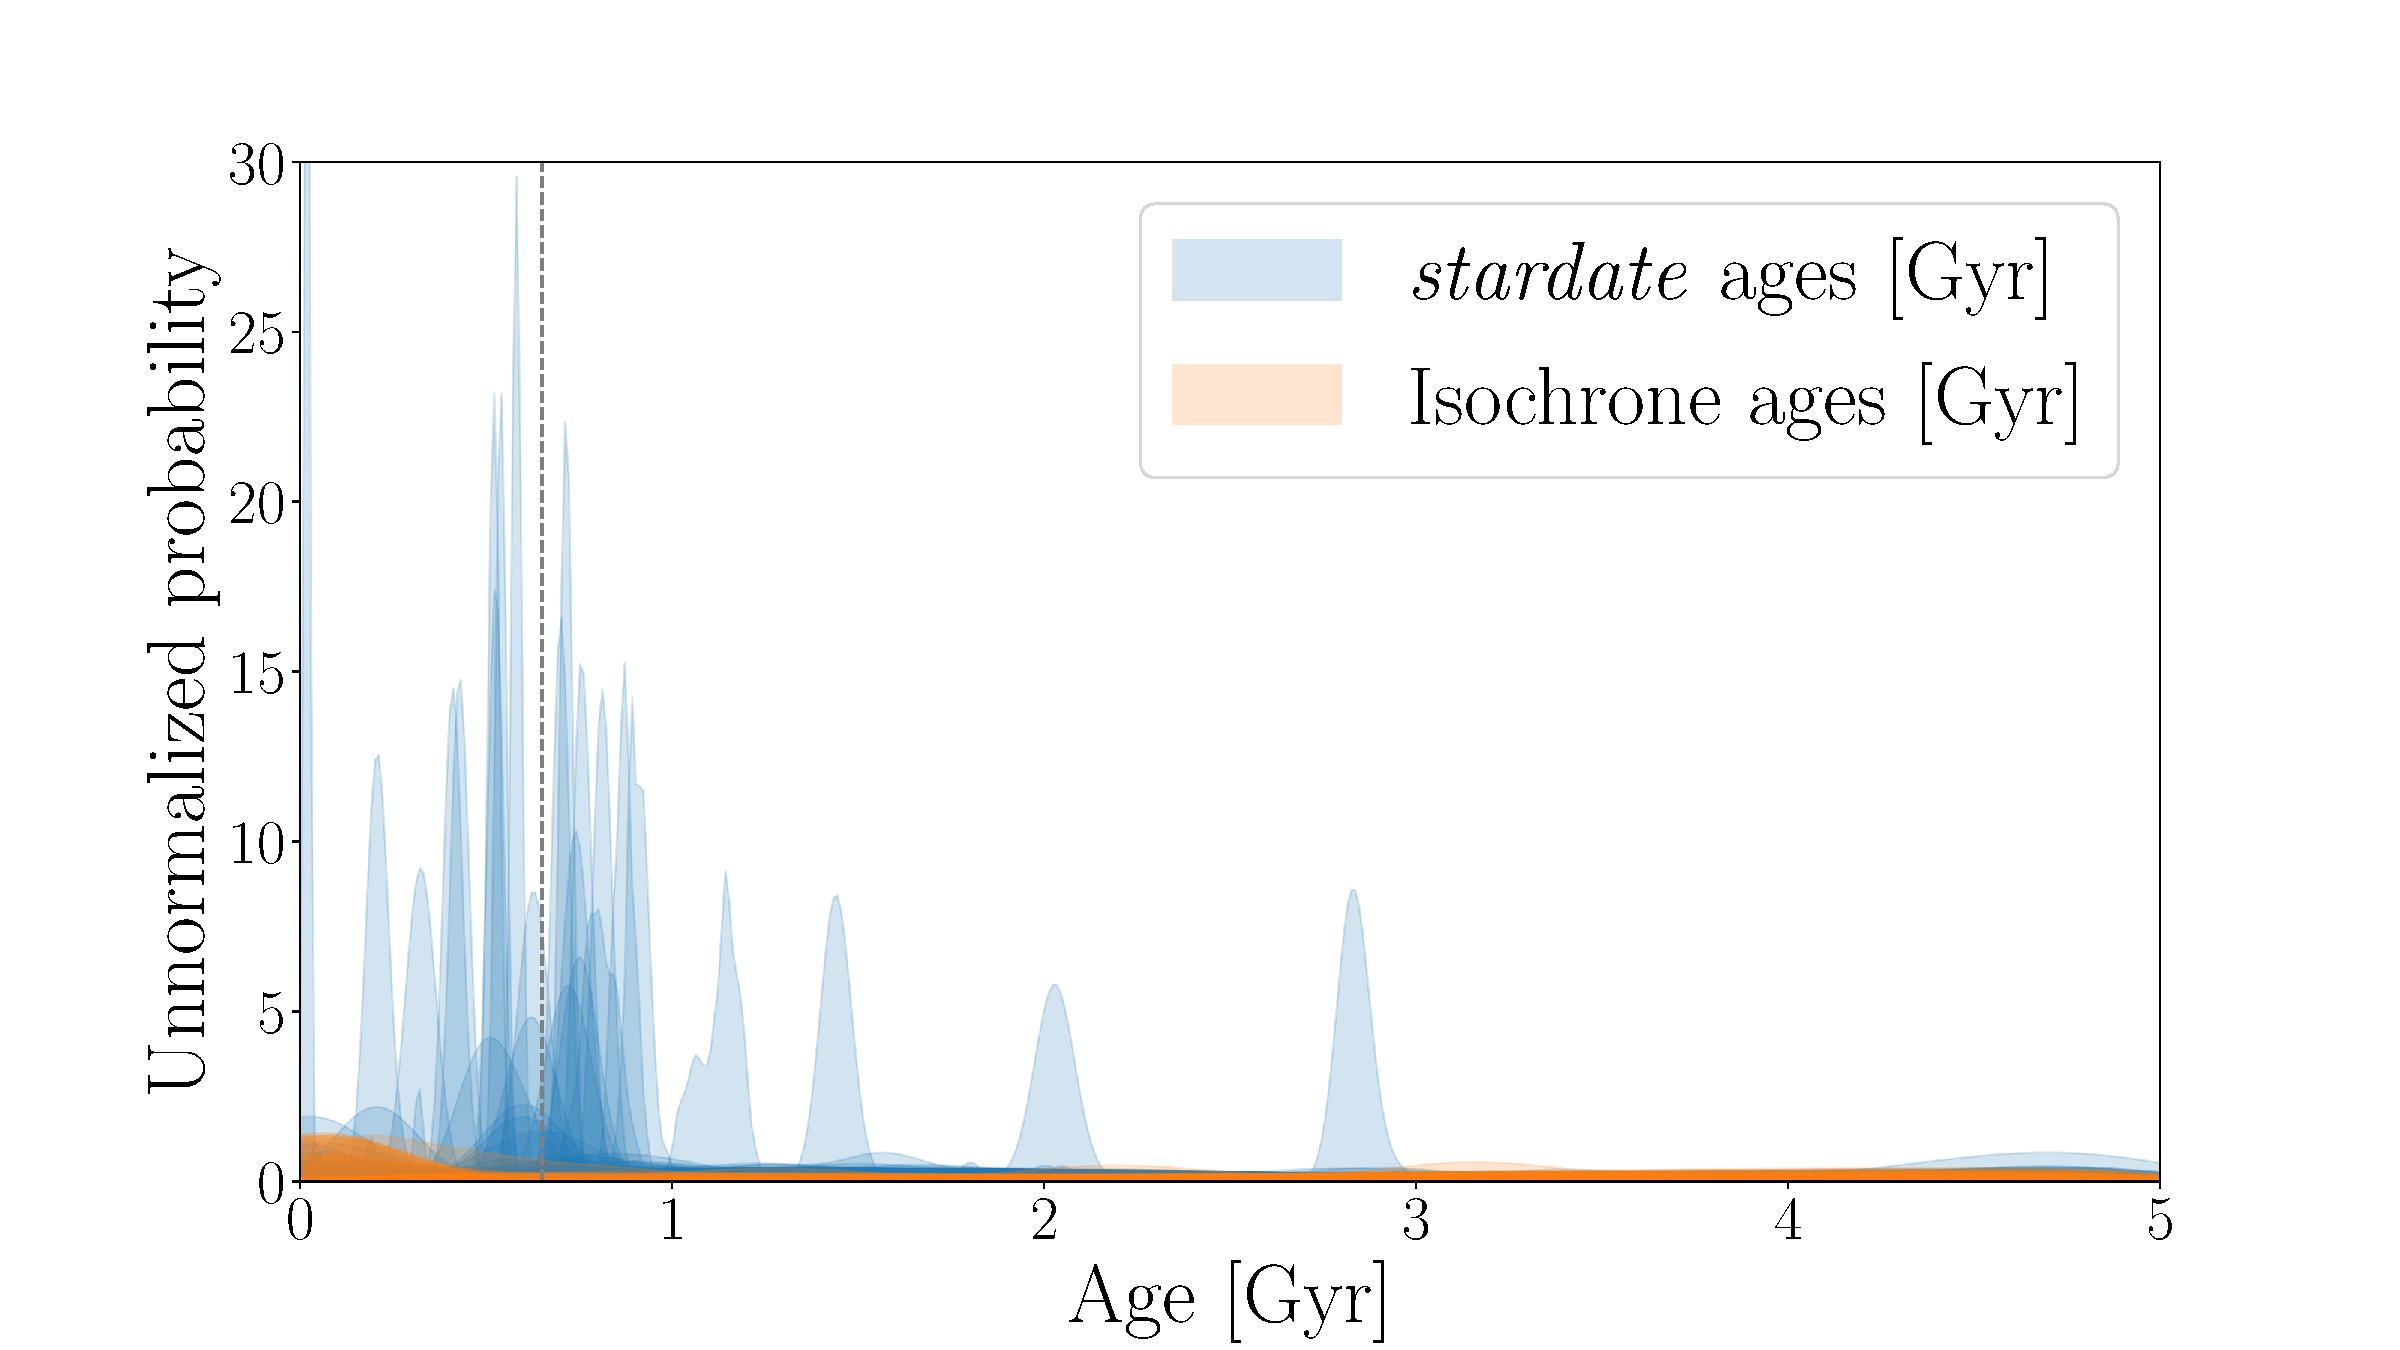
\includegraphics[width=1\textwidth]{praesepe_results}
\label{fig:praesepe_results}
\end{figure}

% % Cutting outliers and limiting color range.
% In order to fit a period-color relation to these data we restricted the sample
% of cluster stars to the color range, 0.56 $<$ \gcolor\ $<$ 3 in order to
% remove early F and late M dwarfs whose rotation periods do not fall on the
% `gyrochronology main sequence'.
% Although it {\it may} be possible to crudely predict the ages of these stars
% (at least the M dwarfs) from their rotation periods, the age-rotation-color
% relation for these stars is very different to the FGK star relations and is
% not the focus of this paper.
% In addition, we removed rapidly rotating stars from the sample since, although
% modeling outliers is important and consequential for gyrochronology in
% general, the goal of this paper is not to produce a perfect gyrochronology
% that reproduces stochasticity in the data, just a simple function that fits
% the rotational main sequence of Praesepe.
% In future we plan to update the gyrochronology models to include M dwarfs,
% and the outlying rapid rotators using a mixture of Gaussians.
% Similarly, we used only Praesepe in this study because the period-color
% relations of each open cluster with rotation periods has a different shape.
% This is likely due to differences in metalicities, incomplete or noisy
% membership lists and differences in rotation period measurement algorithms.
% A global gyrochronology calibration, using all cluster data is planned for the
% future but, again, is beyond the scope of the project presented here.
% The rotation periods of the Praesepe members in the restricted color range and
% with outliers removed are plotted against their \Gaia\ colors in figure
% \ref{fig:Praesepe}.
% We used linear least squares to fit a linear model to Praesepe and the Sun.
% A 4th order polynomial in $\log(G_{BP} - G_{RP})$ and a straight line in
% $\log(\mathrm{Age~[yrs]})$ was fit to reproduce
% $\log(\mathrm{rotation~period~[days]})$.
% \begin{equation}
%     \log(P) = a + b\log(C_G) + c\log^2(C_G) + d\log^3(C_G) + e\log^4(C_G) +
%     f\log(A),
% \end{equation}
% \label{eq:new_gyro}
% were $P$ is period, $C_G$ is \Gaia \gcolor\ color, and A is age.

% %   - Praesepe results: metallicity, mass, distance
% Stellar rotation periods are age-informative and so including them in our
% analysis leads to the more precise measurement of ages.
% However, rotation periods do not carry very much information about the
% metallicity of a star, nor their distance.
% They are also not particularly informative about the mass of a star because,
% even though rotation period depends on both mass and age, stellar mass is
% strongly informed by color and temperature information, so is chiefly
% determined by the stellar evolution/isochrone models.
% However, age, mass and metallicity are correlated: a star can be more blue
% because it is more massive, older or more metal poor and for this reason, if a
% star's age is more tightly constrained, constraints on its mass and
% metallicity will also improve.
% Figures \ref{fig:metallicity} and \ref{fig:mass} show the differences in
% posterior PDFs over metallicity and mass respectively, calculated for Praesepe
% stars where rotation period information is both used (blue posteriors) and not
% used (orange posteriors).
% The black line in figure \ref{fig:metallicity} shows the established
% metallicity of Praesepe \racomment{citation}.
% There is little difference between blue and orange because rotation periods do
% not strongly depend on metallicity or mass (independantly of age).
% However, the precision of mass and metallicity measurements are slightly
% improved due to the fact that age, mass and metallicity are correlated.
% Figure \ref{fig:distances} shows the posterior PDFs over distance to the
% Praesepe cluster.
% In this example of fitting our model to Prasepe data, Since we used \gaia\
% parallaxes, which are extremely informative about distances, more precisely
% constrained ages make a minimal improvement to distances.

%   - Praesepe results: the Praesepe gyro relation
% The results in figure \ref{fig:praesepe_old_model_ages} were produced using a
% gyrochronology relation (equation \ref{eqn:old_gyro}) that was calibrated
% using the Hyades, Coma Berenices and Pleiades clusters, plus the Sun and old
% asteroseismic stars \citep{angus2015}.
% Figure \ref{fig:praesepe_new_model_ages} however, shows the results of
% inferring the ages of Praesepe members with the dedicated Praesepe
% gyrochronology relation of equation \ref{eqn:gyro_age_praesepe}.
% We include these results because we would like to provide an idea of the kind
% of age measurement accuracy that is achievable in the best case: where the
% gyrochronology model perfectly reproduces the data.

%   - Summary
In summary, fitting our new age model to simulated stars and members of the
Praesepe cluster (an open cluster with a precisely measured age from ensemble
isochrone fitting and MS turn-off) demonstrates that using isochrone fitting
{\it alone} to calculate the ages of cool MS field stars results in
extremely imprecise ages, however when gyrochonology is incorporated, the
precision of age measurements increase significantly.

% % The simulation figures
% % iso only
% \begin{figure}
%   \caption{
% The results of a test in which we simulated observable properties of stars
%     with the same model we used to infer their properties.
% In this experiment we used {\it only} isochrone fitting to infer ages;
% we did not use rotation periods/gyrochronology.
%     For results where we used {\it both} stellar evolution models {\it and}
%     gyrochronology, see figure \ref{fig:iso_and_gyro}.
% The true age, used to produce associated observables is shown on the x-axis,
%     and the inferred ages are shown on the y-axis.
% This figure shows the posterior PDFs over stellar age for each of the
%     simulated stars as a `violin plot', where samples from the posterior are
%     plotted vertically as a smooth, symmetric function.
% The widths of these functions indicates the probability density over age:
%     wider regions indicated greater probability mass.
% The median values of the posterior PDFs are plotted as solid horizontal lines.
% This figure demonstrates that when only stellar evolution models are used to
%     infer ages for field MS stars, the resulting predicted ages are extremely
%     imprecise.
% }
%   \centering
%     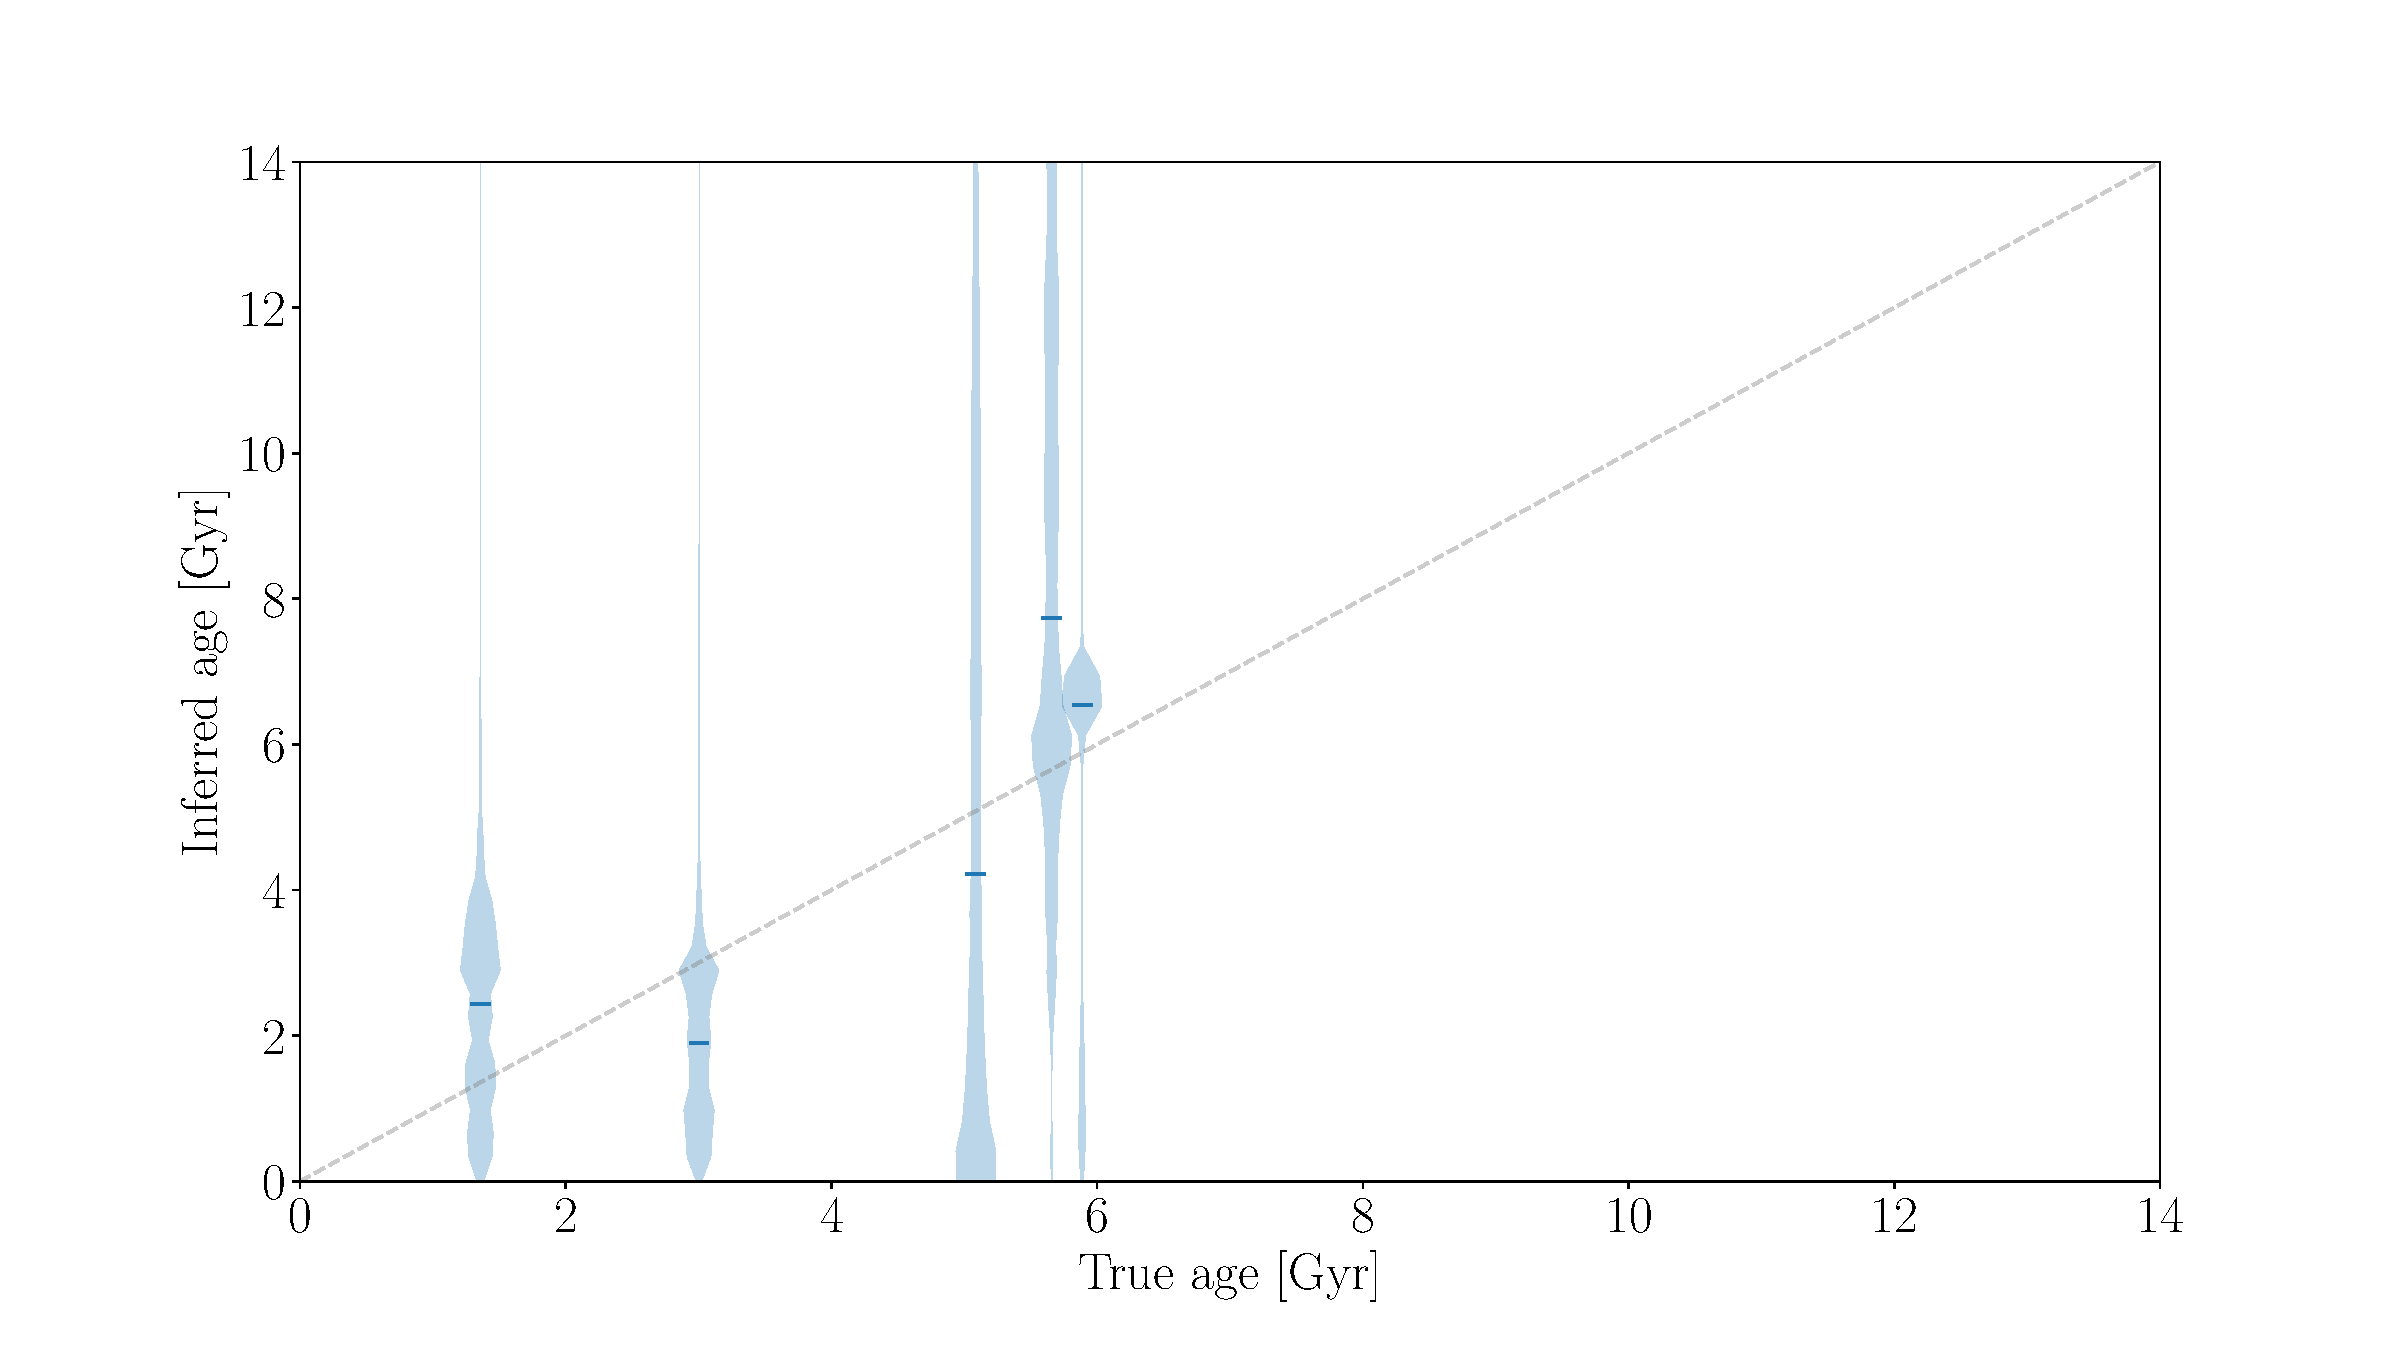
\includegraphics[width=1\textwidth]{../plots/iso_only_violin.pdf}
% \label{fig:iso_only}
% \end{figure}

% \begin{figure}
%   \caption{
% The results of a test in which we simulated observable properties of stars
%     with the same model we used to infer their properties.
%     In this experiment we used both isochrone fitting {\it and}
%     gyrochronology to infer ages.
% For results where we used stellar evolution models {\it only}, see the
%     previous figure (figure \ref{fig:iso_only}).
% The true age, used to produce associated observables is shown on the x-axis,
%     and the inferred ages are shown on the y-axis.
% This figure shows the posterior PDFs over stellar age for each of the
%     simulated stars as a `violin plot', where samples from the posterior are
%     plotted vertically as a smooth, symmetric function.
% The widths of these functions indicates the age probability density: wider
%     regions represent greater probability mass.
% The median values of the posterior PDFs are plotted as solid horizontal lines.
%     This figure demonstrates that when rotation periods (gyrochronology) {\it
%     and} stellar evolution models are used to infer the ages of field MS
%     stars, the resulting predicted ages are much more precise
%     than isochrone fitting can provide alone.
%     \racomment{I am rerunning code to fix the outliers in this figure -- I
%     think it's an initialization issue. I am also planning to combine this
%     figure with the figure above.}
% }
%   \centering
%     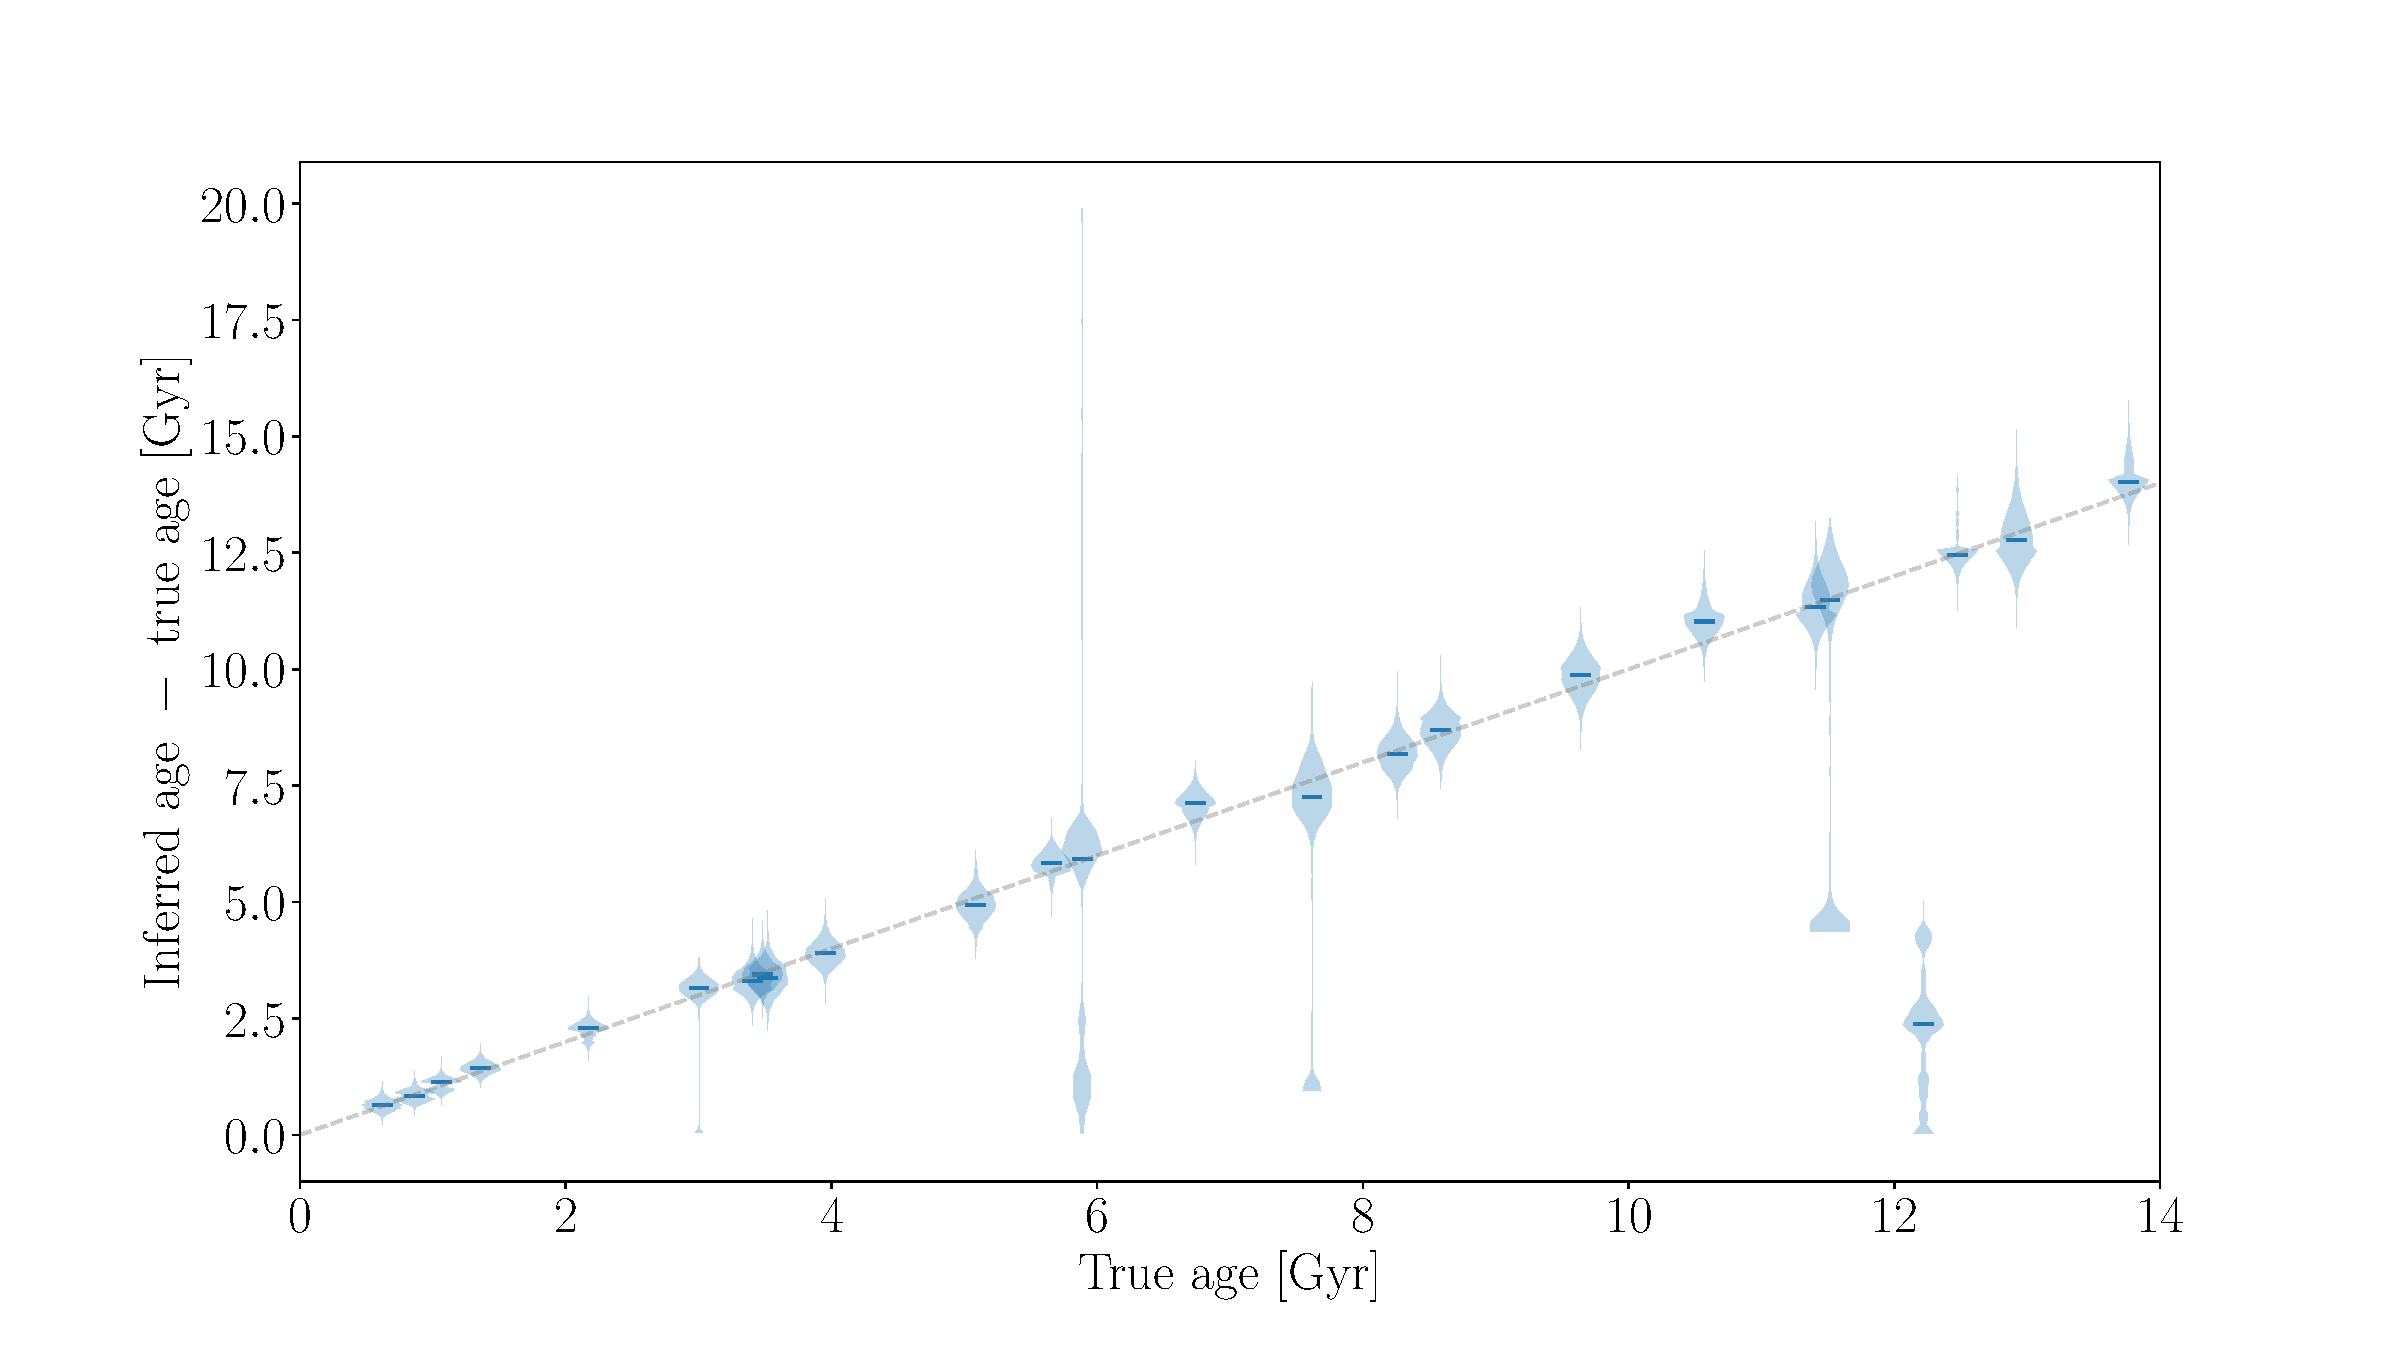
\includegraphics[width=1\textwidth]{../plots/iso_and_gyro_violin.pdf}
% \label{fig:iso_and_gyro}
% \end{figure}

% % The Cluster figure
% \begin{figure}
%   \caption{
% % The rotation periods of stars in open clusters, and the Sun, plotted against
% %     their \Gaia\ colors (\gcolor) in logarithmic space.
% % The result of this fit is plotted on top of the data at the ages of
% %     the cluster stars and the Sun.
%     The rotation periods of Praesepe members and the Sun, plotted against
%     their \Gaia\ colors (\gcolor) in logarithmic space.
%     We fit a linear model to these data in order to predict
%     rotation periods from \gaia\ colors and age.
%     This model consisted of a fourth-order polynomial in $\log_{10}$ color,
%     and a 1st order polynomial (a straight line) in $\log_{10}$ age.
% The result of this fit is plotted on top of the data at the ages of
%     Praesepe and the Sun.
% }
%   \centering
%     \includegraphics[width=1\textwidth]{clusters.pdf}
% \label{fig:clusters}
% \end{figure}


% \begin{figure}
%   \caption{
%     The unnormalized posterior PDFs over the ages of Praesepe stars inferred
%     using an isochrone fitting method (orange) and a joint isochrone fitting
%     and gyrochronology model (blue).
%     MIST isochrones were used for isochrone fitting and the gyrochronology
%     model is shown as solid grey lines in
%     figure \ref{fig:praesepe} \citep{angus2015}.
%     The black line shows the established age of Praesepe (650 Myrs).
%     The blue posterior PDFs are more strongly peaked around the established
%     age for Praesepe than the orange, indicating that gyrochronology is much
%     more informative for these MS stars than isochrone fitting.
%     \racomment{Still need to quantify the improvement. Also need to plot these
%     stars on a CMD, colored by their age uncertainties. Need to make sure
%     there are some Praesepe subgiants in there to test the isochrone fitting.}
% }
%   \centering
%     \includegraphics[width=1\textwidth]{cluster_ages.pdf}
% \label{fig:cluster_ages}
% \end{figure}


% \begin{figure}
%   \caption{
%     The posterior PDFs over metallicity of Praesepe stars inferred using an
%     isochrone fitting method (orange) and a joint isochrone fitting and
%     gyrochronology model (blue).
%     The black line shows the established metallicity of Praesepe (citation).
%     The blue posterior PDFs are
% }
%   \centering
%     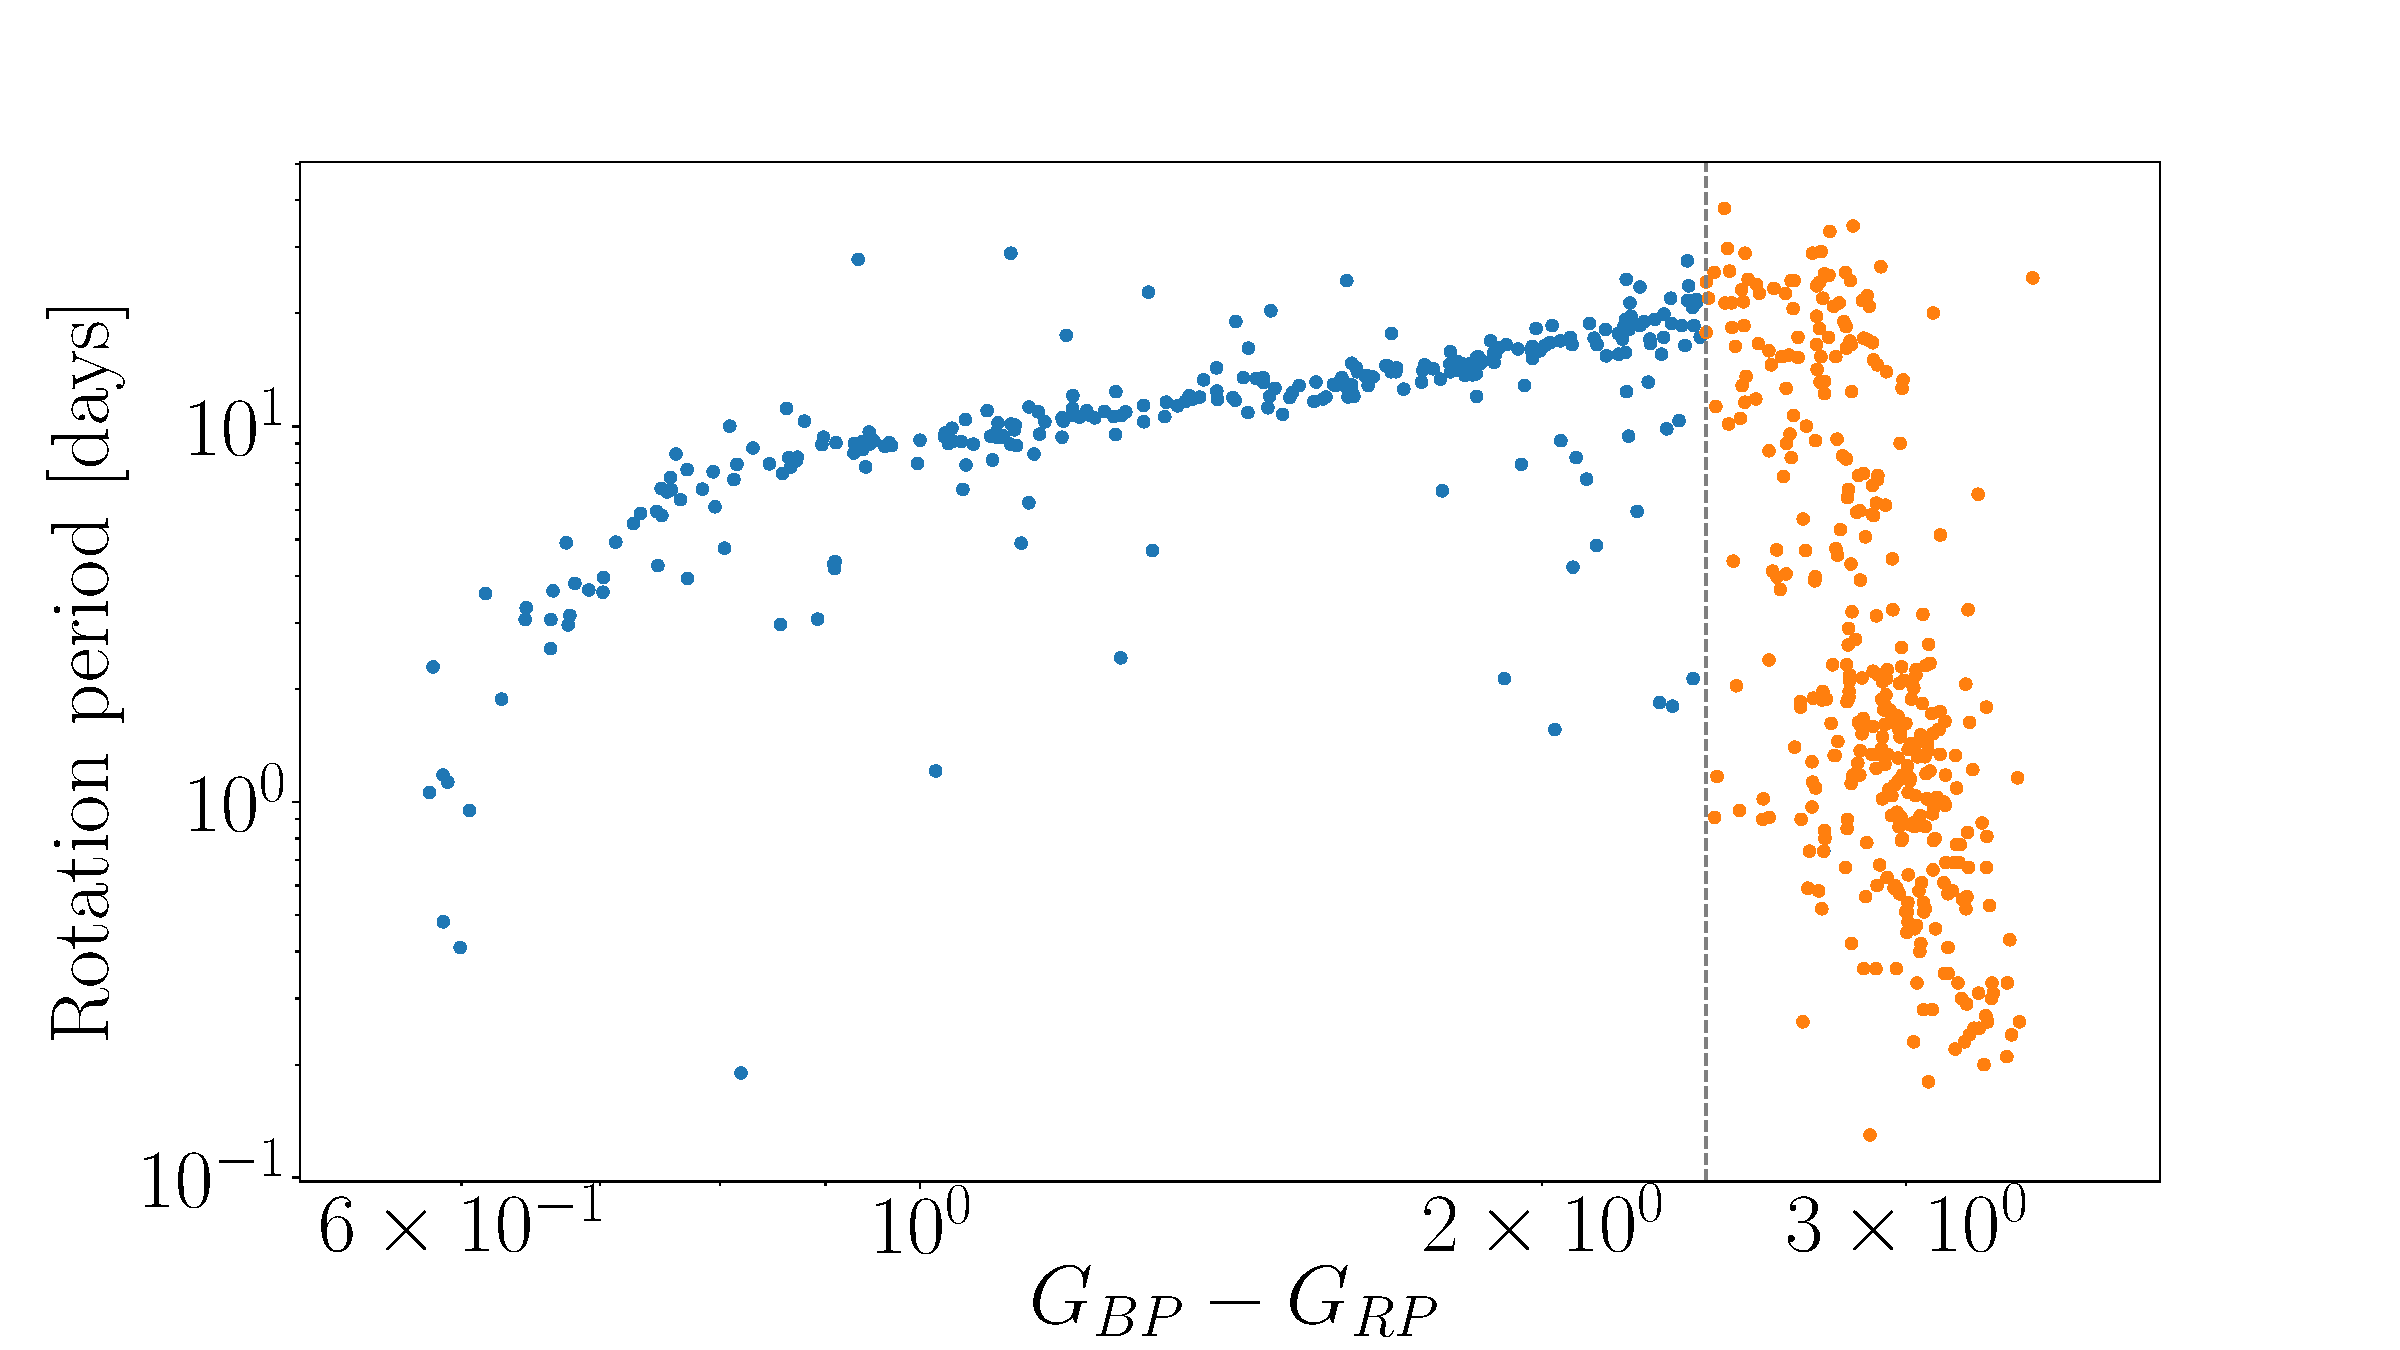
\includegraphics[width=1\textwidth]{praesepe.pdf}
% \label{fig:metallicity}
 % \end{figure}
